\chapter{Diseño e implementación del modelo.}
\epigraphhead [30]{%
  \epigraph{``El hardware es lo que hace a una máquina rápida; el software es lo que hace que una máquina rápida se vuelva lenta"}%
  {Craig S. Bruce, desarrollador.}%
}




	La lógica del programa se ha desarrollado de la manera más óptima y flexible, posible facilitando la ampliación de las funcionalidades del mismo así como la  reutilización de código en el futuro. Para ello es importante la modularización de cada parte, en este capítulo se explica como se ha realizado esa tarea en el programa y su funcionamiento interno.

	\section{Modulos que forman el programa.}
		Un módulo en Python es un conjunto de funciones, clases u otros módulos que pueden ser importados en otros módulos o clases dando flexibilidad al código programado. El programa está formado por tres módulos principales llamados \emph{classes}, \emph{GUI}, y \emph{utils}.
	\begin{itemize}
		\item \emph{classes} contiene los objetos que utiliza el modelo para funcionar.
		\item \emph{GUI} contiene todos los objetos del interfaz gráfico.
		
		\item \emph{utils} contiene funciones o clases con propósitos específicos ubicadas aquí para liberar las clases principales de código o porque pueden ser de interés en diversas partes del programa.
	\end{itemize}

		\begin{figure}[H]
		  \centering
		  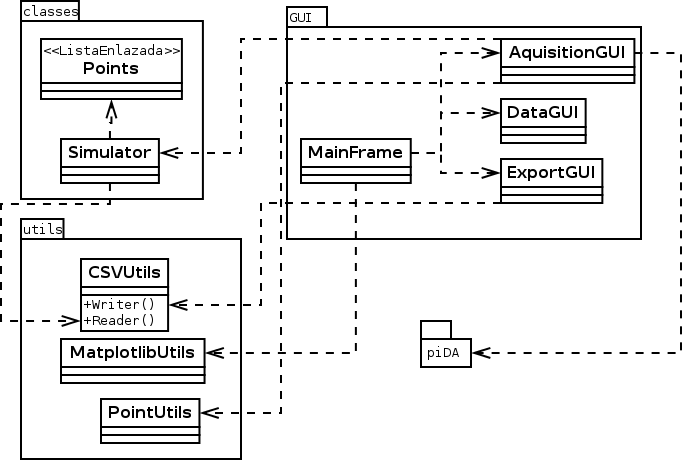
\includegraphics[width=1\textwidth]{img/classes.png}
		  \caption{Diagrama de clases y sus dependencias..}\label{fig:diag-classes}
		\end{figure}

	Las clases mostradas en el diagrama de la \autoref{fig:diag-classes} se detallan a continuación:
	
	\subsection{Módulo \emph{classes}.}\label{subsec:classes}
		\begin{itemize}
			\item Points.py: Esta clase contiene una lista enlazada de puntos (x,y) con un iterador infinito: Cuando llega al final de la lista el siguiente elemento vuelve a ser primero de la lista pero con el valor $ x_{i} $ sumado al $ x_n $ y dejando $ x_y $ igual. Al alcanzar de nuevo el final de la lista, el valor sumado $ x_n $ se dobla para mantener la continuidad de la línea de puntos.
			\item Simulator.py: Esta clase contiene el simulador programado para realizar pruebas cuando la interfaz piDA de adquisición de datos aún no estaba operativa. Su funcionamiento está explicado en la \autoref{sec:sim}). El simulador implementa el diseño acordado en la \autoref{subsec:especificacion_piDA} para que una vez el prototipo estuviese preparado para incluirse en el software la transición fuese directa.
		\end{itemize}
		El módulo incluye además las clases no desarrolladas:
		\begin{itemize}
			\item Acquisition.py: Diseño rudimentario del interfaz de adquisición de datos discontinuado.
			\item Graph.py: Clase que representa una gráfica con sus datos, propiedades y vistas, con objetivo de poder ser guardada como formato propio o dentro de un fichero de proyecto.
			\item Histogram.py: Idéntica a la clase Graph pero esta vez con un histograma para abordar la solución del laboratorio de radiactividad.
			\item Project.py: Clase que representa un proyecto, con sus datos y gráficas con objetivo de guardarlo en un fichero y poder recuperar el trabajo en otro momento.
		\end{itemize}
	
	\subsection{Módulo \emph{GUI}.}	
		Dado a que el diseño del interfaz gráfico está explicado en su propio \autoref{chap:GUI}, aquí solo se explican las funciones correspondientes a la parte del modelo.
		\begin{itemize}
			\item AcquisitionGUI.py: Implementa un panel con los controles para manejar un interfaz de adquisición o simulador creado dentro del mismo. Es una de las clases clave ya que incluye la lógica que envía los datos a la gráfica de la ventana principal, explicada en la \autoref{subsec:act_datos}.
			
			Al instanciar esta clase se pasa un número de canal como argumento que intenta inicializarse en la interfaz piDA, si no es posible obtenerlo, el panel queda desactivado. Esto es útil por ejemplo si piDA soporta varios interfaces de adquisición con distinto número de canales cada uno. Por ejemplo, el primer prototipo (\autoref{sec:primer_prototipo}) solo soportaba dos canales.
			
			\item DataGUI.py: Implementa un panel para visualizar los datos adquiridos. \autoref{sec:gui_DataGUI}.
			\item ExportGUI.py: Implementa un panel para exportar los datos adquiridos. \autoref{sec:gui_ExportGUI}.
			\item MainFrame.py: Implementa la ventana principal. \autoref{sec:gui_mainframe}.
			
			Aquí están las funciones encargadas de controlar el refresco automático y manual de la gráfica y la petición de datos a los distintos módulos activos para la misma.
		\end{itemize}
	
	\subsection{Módulo \emph{utils}.}
	\begin{itemize}
		\item CSVUtils.py: Contiene dos clases Reader, y Writer las cuales sirven para leer o escribir ficheros CSV.
		\begin{itemize}
			\item La clase Reader recibe una ruta de archivo CSV en el formato del programao o del software del laboratorio termodinámica y física aplicaada \emph{DataStudio}. Reconoce el título, cabeceras de las columnas y cada par de datos $ x $ e $ y $, los cuales los incluye en un lista de tipo Points (ver \autoref{subsec:classes}).
		
			\item La clase Writer recibe una ruta para crear el fichero y provee de los métodos para escribir en él una o más filas con el formato del programa y codificación UTF-8.
		\end{itemize}		
		
		\item MatplotlibUtils.py: Contiene tres funciones para tratar con la API interna de Matplotlib de colores de líneas. Se ha añadido además la opción de no dibujar la línea.
		\begin{itemize}
			\item La función IntToCharColor recibe un entero del 0 al 7 y devuelve un carácter de color para Matplotlib. Si se recibe un número fuera de ese rango la línea no se dibuja (carácter 'z'). Los códigos y el color que representa soportados por Matplotlib son, en orden:\\
			b: blue\\
			g: green\\
			r: red\\
			c: cyan\\
			m: magenta\\
			y: yellow\\
			k: black\\
			w: white
			
			\item IntToColor recibe un entero y devuelve una cadena de carácteres con su nombre en lenguaje natural, el orden y los nombres se pueden ver en la lista del apartado anterior. Cualquier valor fuera del rango retorna la cadena ``None''.
			
			\item GetColorList retorna una lista con los colores soportados por Matplotlib en lenguaje natural.
		\end{itemize}
		
		\item PointUtils.py Contiene el método PointsToDoubleLists que recibe una lista de puntos en formato $ (x_0,y_0),(x_1,y_1),(x_2,y_2)...(x_n,y_n) $ y retorna dos listas: Una con todas las $ x $ ($ x_0,x_1,x_2...x_n $) y otra con todas las $ y $ ($ y_0,y_1,y_2...y_n $). La librería Matplotlib requiere para dibujar que se le entreguen los puntos $ x $ e $ y $ por separado, por tanto se necesita hacer una conversión.
	\end{itemize}
	
	\section{Lógica de control de la gráfica.}
	
	

		
	\subsection{Actualización de los datos.}\label{subsec:act_datos}
	La actualización de los datos de la gráfica se realiza en un proceso de dos pasos:
	\begin{description}
		\item[Obtener los datos de cada canal.] Se llama secuencialmente a cada canal activo o con datos para pintar y se le pide que envíe sus datos a la gráfica. Ésta llamada corre sobre un hilo diferente al que se está utilizando en ese canal para obtener datos, por tanto se han implementado semáforos de tipo mútex para la sincronía entre hilos concurrentes. La llamada espera a que no se estén utilizando los datos en el módulo para obtener una copia de los mismos, que la convierte mediante PointsToDoubleLists en datos que puede enviar a la gráfica. El color de la línea también se especifica en este instante, por lo que puede ser cambiado en cualquier momento de la adquisición. Los gráficos serán mostrados en el próximo redibujado de la gráfica.
		

		En la \autoref{fig:diag-enviodatos} se puede ver un diagrama de cómo se inicia el proceso desde ``RefreshGraphOnce'' en el la clase de la ventana principal.
		
					\begin{figure}[H]
		  \centering
		  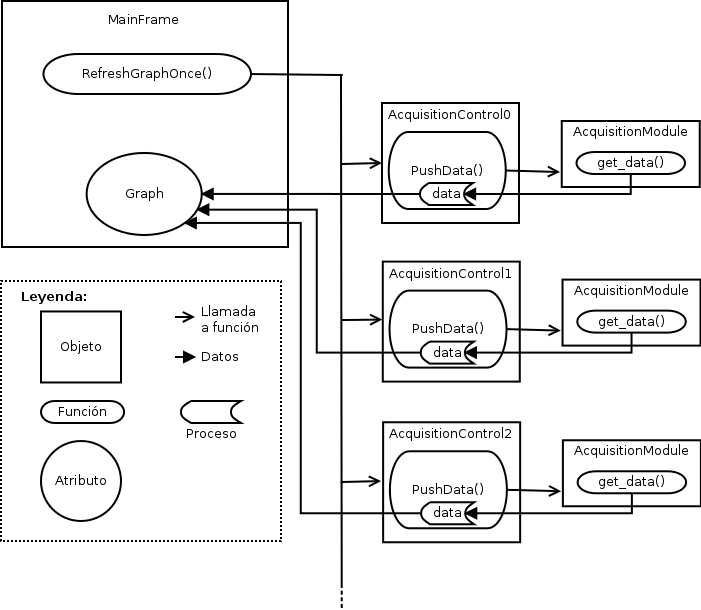
\includegraphics[width=1\textwidth]{img/graph-refresh_diagram.png}
		  \caption{Diagrama de envío de datos a la gráfica.}\label{fig:diag-enviodatos}
		\end{figure}
		
		\item[Redibujado de la gráfica.] La primera implementación de esta tarea fue un redibujado total del lienzo de la gráfica, esto incluía los ejes, títulos e información que no necesitaba modificarse. Este modo resultaba muy intensivo de CPU y un verdadero problema si se deseaba realizar una actualización de datos más o menos frecuente, por tanto se buscó una optimización para el mismo.
		
		La optimización encontrada forzaba el cambio de gran parte de la lógica de funcionamiento del programa, por lo que se realizaron tests de rendimiento comparando uno y otro sistema. Los resultados mostraron una mejora del 333\% con respecto al método inicial y reduciendo la carga en la CPU significativamente, haciendo obligatoria la implementación de la misma. 
		
		El funcionamiento de esta optimización se basa en la actualización de únicamente del cuadro dónde se dibujan las líneas previa a una restauración del mismo a un estado anterior guardado. De este modo, al iniciar una adquisición de datos se toma el estado de la gráfica y en cada refresco se restaura este estado, y acto seguido se dibujan las líneas de nuevo, con los nuevos valores ya preparados. En la \autoref{fig:diag_refresc} viene una representación de este proceso.
	
		Esta tarea se realiza tras obtener los datos de cada uno de los canales como se ha explicado en el apartado anterior, pero la actualización de un elemento del interfaz gráfico requiere que éste se ejecute sobre el hilo principal, por lo que se llama a esta función desde allí, pudiendo crear pequeños bloqueos si la cantidad de datos a dibujar es muy grande.
	
		
		\begin{figure}[H]
			\centering
		  	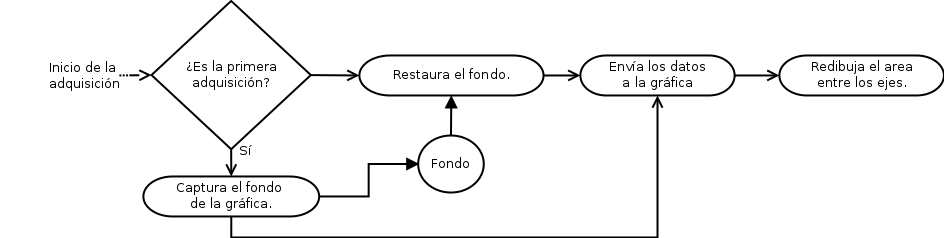
\includegraphics[width=1\textwidth]{img/graph_redraw-diagram.png}
  			\caption{Diagrama de refresco selectivo de la gráfica.}\label{fig:diag_refresc}
		\end{figure}
	\end{description}


	\subsection{Actualización automática.}
		Una función básica para poder ver los datos a la vez que se toman a través del interfaz de adquisición es que la gráfica se vaya actualizando automáticamente. El diseño del sistema es muy sencillo: Cuando es activado, comienza un hilo donde un bucle llama en el intervalo que ha especificado el usuario a la función de actualizar la gráfica. Cuando se desactiva esta función, el bucle finaliza, y con él el la ejecución del hilo.
		
				\begin{figure}[H]
			\centering
		  	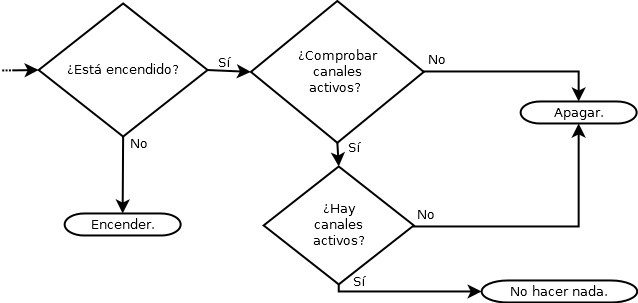
\includegraphics[width=1\textwidth]{img/toggle_graph.png}
  			\caption[Función de encendido o apagado del refresco automático de la gráfica.]{Función de encendido o apagado del refresco automático.}\label{fig:diag_toggle}
		\end{figure}
		
		Ha supuesto un pequeño desafío programar cuándo esta función ha de activarse o desactivarse, ya que su estado encendido o apagado depende de un control de usuario general, y diversos canales ejecutándose en diferentes hilos de ejecución. Se ha creado una sola función \emph{ToggleGraphRefreshing} encargada de activarlo o desactivarlo. La función usada sin ningún argumento hace su función natural: si está apagado lo enciende, si está encendido lo apaga. En cambio si se especifica que compruebe los canales pasando como argumento check\_channels=True comprueba que no haya ninguno activo antes de apagar. En la \autoref{fig:diag_toggle} se puede ver la representación de este proceso.



	\section{El simulador.}\label{sec:sim}
	Durante el transcurso del proyecto desarrolló un simulador de interfaz de adquisición de datos para poder probar los elementos y no retrasar el desarrollo de esta parte. 
	
	La lógica de funcionamiento del mismo es simple: como su propio nombre indica, ha de simular el funcionamiento de un interfaz de adquisición. Por tanto se ha adoptado el diseño descrito en la \autoref{subsec:especificacion_piDA} para que además llegado el momento de integrar el prototipo desarrollado en el proyecto paralelo no haya que modificar la lógica del programa.
	
	\subsection{Lógica de funcionamiento.}
		El simulador dispone de una lista interna de puntos que es el ``origen de datos''. Durante la adquisición, cada elemento de esta lista se copia a la frecuencia especificada a otra lista accesible mediante el interfaz.
		
		Para ello, al iniciarse se crea un hilo de ejecución donde un bucle copia los valores de una lista a otra. Al final de cada bucle se comprueba si se ha ordenado detener la adquisición o si ha de continuar. Si es la segunda opción, se espera la inversa de la frecuencia de muestreo antes de volver a copiar el siguiente valor de la lista iterada, como se puede ver en la  \autoref{fig:diag_simulator}.
\begin{figure}[H]
			\centering
		  	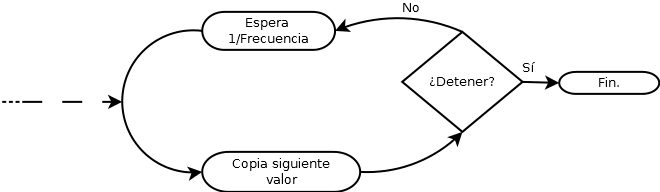
\includegraphics[width=1\textwidth]{img/diag_simulator.png}
  			\caption[Función de encendido o apagado del refresco automático de la gráfica.]{Función de encendido o apagado del refresco automático.}\label{fig:diag_simulator}
		\end{figure}
		
	\subsubsection{El origen de los datos.}
			El simulador obtiene sus datos de un fichero CSV que se carga con clase Writer descrita en apartados anteriores, obteniendo así una lista iterable infinita Points.
			
			Se ha tomado la decisión de tomar datos reales procedentes de un fichero en lugar de valores generados aleatoriamente o por una función matemática para que éstos sean lo más parecidos a los que se van a manejar con el prototipo. Además, de este modo se ha desarrollado un módulo de importación de ficheros CSV útil en el futuro.
		
	\section{Los distintos hilos de ejecución.}
	El software está programado concurrentemente, con los problemas de sincronía que  esto puede ocasionar si no son tratados adecuadamente. 

	El programa ejecuta un hilo principal donde el interfaz gráfico es ejecutado, y pueden crearse hasta cinco hilos más, esto es uno por cada canal adquiriendo datos y otro controlando la actualización y obtención de datos de cada uno de los canales.
	
	El punto más susceptible para que un error de sincronía suceda es en el momento que el hilo correspondiente a la obtención de datos de cada canal accede a la lista donde éstos están guardados a la vez que se está almacenando un valor. Esto provocaría por ejemplo que en la lista esté escrito el valor $ x $ pero no el $ y $, por tanto enviando a la gráfica una lista de puntos $ x_n $ con un tamaño diferente al de $ y_n $, provocando un fallo en la gráfica.
	
	Se ha solucionado este problema de sincronización mediante el uso de secciones críticas controladas por semáforos binarios (\emph{mútex}) en cada interfaz de adquisición. De este modo nunca se accederá a la lista de datos de un interfaz de adquisición si este se encuentra escribiendo sobre él, si no que, como muestra el diagrama de la \autoref{fig:diag_sincronia}, esperará a que el semáforo de dicho interfaz esté libre para tomarlo, obtener los datos y dejarlo libre de nuevo.
	
	\begin{figure}[H]
			\centering
		  	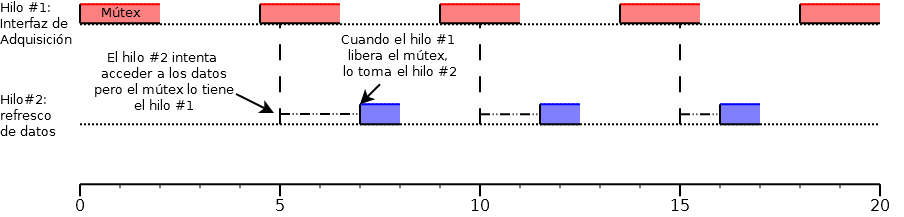
\includegraphics[width=1\textwidth]{img/diag-sincronia.png}
  			\caption{Diagrama de sincronización entre hilos.}\label{fig:diag_sincronia}
		\end{figure}
	
	
\section{Otras funciones integradas: Instalador.}
	Junto con el resto de ficheros se incluye un ``setup.sh'' que configura el sistema para la ejecución del programa. 
	
	Este fichero de comandos instala las librerías de las que se depende \emph{WxPython} y \emph{Matplotlib} del repositorio oficial de Raspbian. Además, obtiene del repositorio de Git la versión más actual del interfaz de adquisición de datos piDA y lo instala en el sistema.
	
	Por tanto, la replicación de este programa en las distintas estaciones es tan sencillo como ejecutar los siguientes comandos:\\
	\indent \$ git clone https://github.com/dmcelectrico/PFC.git \\
	\indent \$ ./PFC/setup.sh \\